\clearpage
\section{النماذج}
\label{sec:builder-feature-forms}

النموذج صفحة أسئلة يعبّئها موظف أو مقدّم طلب، مثل طلب إجازة أو استمارة زيارة. وتنشئ النماذج وتنشر إصداراتها من صفحة «النماذج»، ويمكن أن يكتب النموذج إجاباته في نوع سجلات، وأن يكون له مسار حالات واعتماد. ويعمل الناس دائماً على الإصدار المنشور، بينما تعدّل أنت مسودة جديدة دون أن تؤثر فيهم.

\textbf{المسار ومن يستخدمه:} «ادوات البناء» ← «الأساسية» ← «النماذج». يستخدمها من يملك صلاحية النماذج لتصميم طريقة جمع الطلبات.

\begin{rcnote}[مثال: شركة الأفق]
يبني مسؤول النظام نموذج «طلب زيارة فرع» يسأل عن الفرع والموعد والغرض، ويجعله يكتب الإجابات في «طلبات الزيارة» عند اعتماد سارة الخطيب للطلب، فيعبّئه عمر حداد دون أن يفتح نوع السجلات نفسه. ويبدأ النموذج من ①.
\end{rcnote}

\begin{figure}[H]
\centering
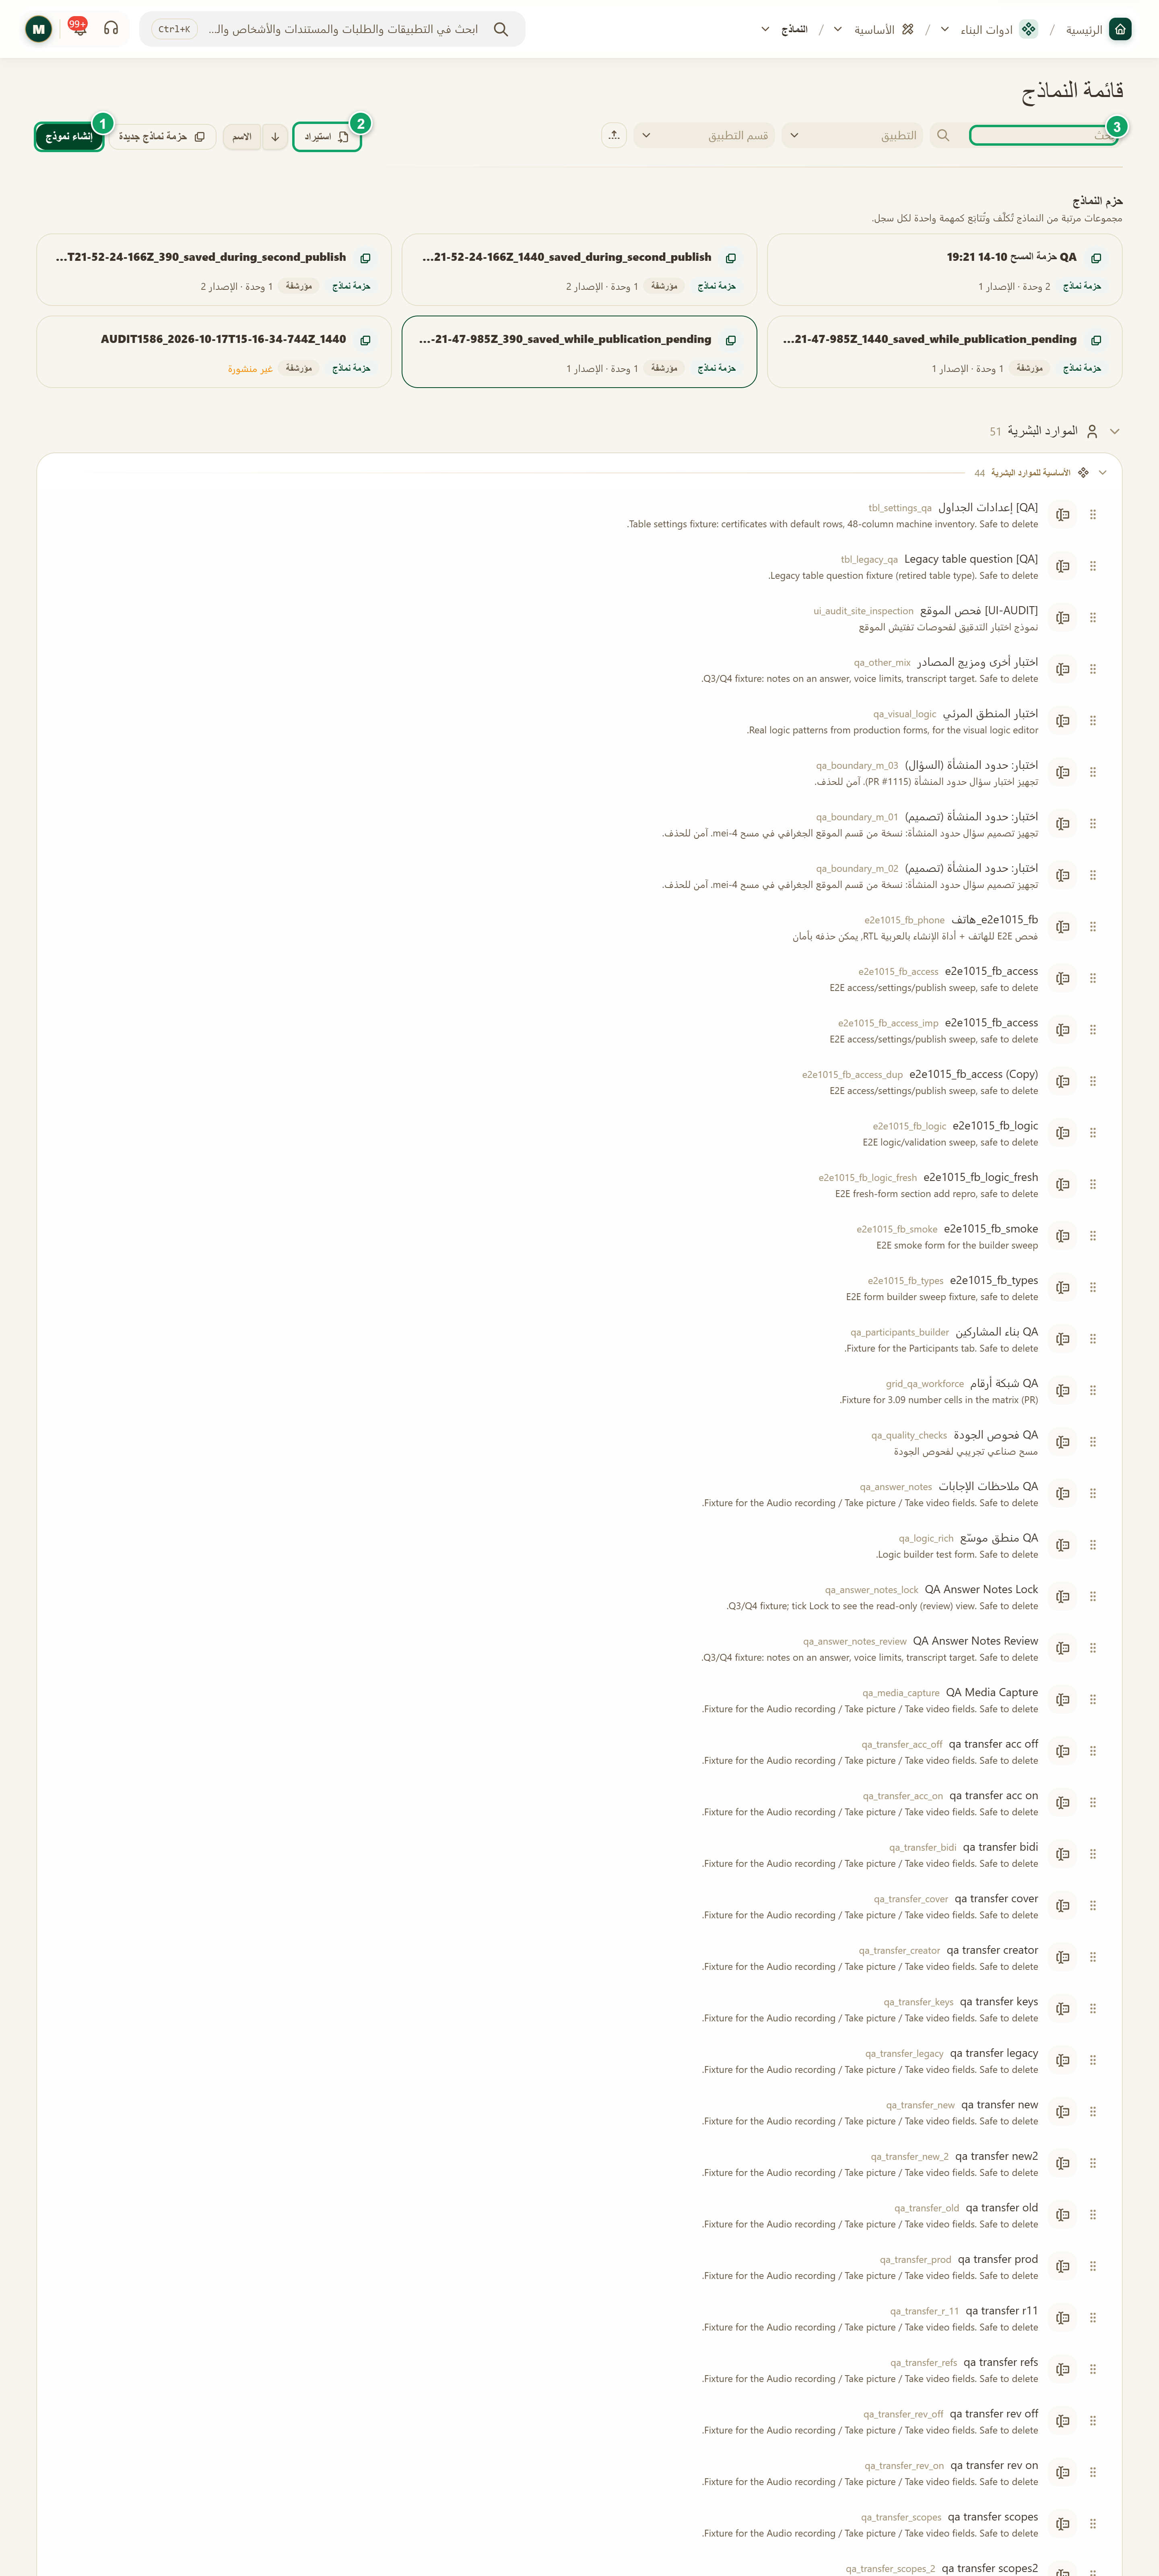
\includegraphics[width=0.95\linewidth,height=0.72\textheight,keepaspectratio]{figures/screens/ch06-forms-ar.png}
\caption{صفحة «النماذج»}
\label{fig:builder-forms-screen}
\shotnote{تعرض الصفحة النماذج مجمّعة حسب التطبيق والقسم مع عدد الطلبات لكل نموذج. والنماذج الظاهرة نماذج اختبار في test2. ① «إنشاء نموذج»: يبدأ نموذجاً جديداً. ② «استيراد»: يُنشئ نموذجاً من ملف مُصدَّر. ③ البحث: يجد النموذج بالاسم.}
\end{figure}


\begin{table}[H]
\centering
\caption{قائمة النماذج}
\label{tab:builder-forms-list}
\begin{tabularx}{\linewidth}{R{3.6cm} Y}
\rcHeaderRow
\thh{الجزء} & \thh{المحتوى والإجراء}\\
إنشاء نموذج & يطلب «اسم النموذج» و«كود النموذج» و«الاختصار المرجعي» والتطبيق والقسم، ثم يفتح المنشئ.\\
القائمة & النماذج مجمّعة حسب التطبيق والقسم، مع البحث والترتيب وعدد الطلبات، وإجراءات «نسخ» و«تصدير النموذج» و«حذف النموذج».\\
استيراد & يُنشئ نموذجاً من ملف مُصدَّر سابقاً.\\
حزم النماذج & مجموعات مرتبة من النماذج تُكلَّف وتُتابَع كمهمة واحدة لكل سجل.\\
\end{tabularx}
\end{table}

\begin{table}[H]
\centering
\caption{أدوات منشئ النموذج}
\label{tab:builder-forms-editor}
\begin{tabularx}{\linewidth}{R{3.6cm} Y}
\rcHeaderRow
\thh{الأداة} & \thh{ماذا تفعل؟}\\
الأسئلة & تضيف الأسئلة من مجموعات: نص، واختيار، وأرقام وتقييم، وتاريخ ووقت، وموقع، والملفات والوسائط، وأخرى؛ مع أقسام وصفحات ونص كتابي.\\
القواعد & كل ما يُظهر سؤالاً أو يخفيه أو يقفله أو يلزم به أو يحسبه أو يتحقق منه، في قائمة واحدة.\\
الوصول & من يستطيع الوصول إلى كل رد، وماذا يستطيع أن يفعل به: من يبدأ النموذج، أو أشخاص ثابتون، أو أشخاص تحددهم الإجابات.\\
المسار & «مسار الطلب»: الحالات والمراحل التي يراها مقدّم الطلب، والانتقالات بينها، وخطوات الموافقة.\\
السجلات & السجلات التي يقرأ منها النموذج ويكتب إليها، ومتى يكتب: «عند الاعتماد» أو «عند الإرسال».\\
إسناد & خطط تكلّف أشخاصاً بتعبئة النموذج لسجلات معينة، وتظهر بعد حفظ النموذج.\\
الإصدارات والإعدادات & «سجل الإصدارات» لكل إصدار، والإعدادات مثل الترقيم ومستند PDF والروابط المملوءة مسبقاً.\\
اختبار النموذج ونشر & يفتح مساحة اختبار معزولة تجرّب فيها النموذج بصفة عضو، ثم «نشر» يجعل المسودة الإصدار المنشور.\\
\end{tabularx}
\end{table}

\begin{figure}[H]
\centering
\begin{tikzpicture}[node distance=0.5cm]
\node[stepBox] (a) {\RL{إنشاء نموذج}};
\node[stepBox,below=of a] (b) {\RL{الأسئلة والقواعد}};
\node[stepBox,below=of b] (c) {\RL{الوصول والمسار والسجلات}};
\node[stepBox,below=of c] (d) {\RL{اختبار النموذج}};
\node[stepBox,below=of d] (e) {\RL{نشر}};
\draw[flowsTo] (a) -- (b);
\draw[flowsTo] (b) -- (c);
\draw[flowsTo] (c) -- (d);
\draw[flowsTo] (d) -- (e);
\end{tikzpicture}
\rclegend
\caption{من الفكرة إلى نموذج منشور}
\label{fig:builder-forms-flow}
\shotnote{يرتّب المخطط بناء النموذج من محتواه إلى سلوكه: الأسئلة أولاً، ثم من يصل إلى الرد وأين تذهب الإجابات. ويأتي الاختبار قبل النشر لأن مساحة الاختبار معزولة، فتكشف الخطأ دون أن يصل إلى أحد؛ أما النشر فيجعل الإصدار متاحاً لكل من يعبّئ النموذج.}
\end{figure}

\subsection{خطوات العمل والتحقق}
\begin{enumerate}
\item افتح «النماذج» واضغط «إنشاء نموذج»، ثم اكتب الاسم والكود والاختصار واختر التطبيق والقسم.
\item أضف الأسئلة، واختر لكل منها نوعاً يناسب الإجابة، ثم أضف القواعد عند الحاجة.
\item افتح «الوصول» لتحدد من يرى الردود، و«السجلات» إن أردت أن تُكتب الإجابات في نوع سجلات.
\item اضغط «اختبار النموذج» وعبّئه كاملاً، ثم اضغط «نشر».
\end{enumerate}

\textbf{تحقق ومعالجة المشكلة:} يجب أن تظهر رسالة «تم نشر النموذج بنجاح»، وأن يظهر الإصدار «منشور» في «سجل الإصدارات». فإذا تحوّل زر النشر إلى «إرسال للاعتماد»، فمؤسستك تشترط اعتماد النشر، وسيُنشر النموذج بعد موافقة المعتمد. وإذا لم تُكتب الإجابات في السجل، فافتح «السجلات» وتأكد من موافقة مسؤول نوع السجلات على كتابة النموذج فيه.
